\section{Ejercicio 5}
\subsection{Introducción}

Se implementó un sumador de dos números de un dígito en BCD, expresando la salida como un número de dos dígitos, también en BCD.
Para ésto, primero se realizó un análisis sobre la suma en este formato, y luego se implementó en un circuito.\\
Se tienen entonces dos números en BCD, que son dos dígitos menores a 9 (pues están en dicho formato). Se realiza una suma convencional en binario. Seguidamente, se compara con 9, ya que si la suma es menor o igual a éste, está representado automáticamente en BCD.
Si la suma es mayor a 9, se le debe sumar un offset de 6 para obtener un 1 en el dígito más significativo, y así, el resultado final. 
El offset de 6 se debe a que en binario, se puede representar como máximo el número 15; en BCD, por otro lado, hasta el 9.
La diferencia entre ambos es de 6, por lo que si queremos que 9+1=10 ($10_{10}=1010_2=0001~~0000_{BCD}$), tenemos que sumar 6
para que $1010_2$ se convierta en  $1~~0000_{BCD}$.
\subsection{Circuito lógico}
Con este razonamiento, se realizó la siguiente implementación:
\begin{figure}[H]
    \begin{center}
        \caption{Circuito lógico del sumador de dígitos BCD.}
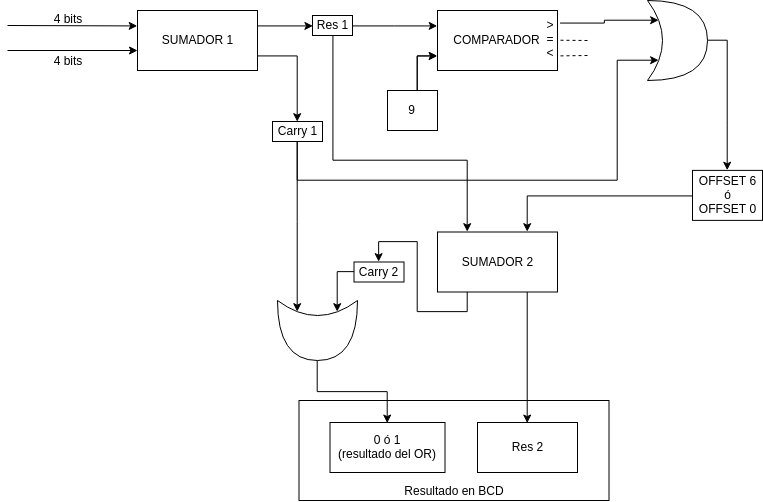
\includegraphics[scale=0.5]{circuito.png}
    \end{center}
\end{figure}

Se puede ver de manera sencilla la lógica que se siguió para el sumador pedido. El resultado final serán dos nibbles. El nibble más significativo es el OR entre los carry de ambos sumadores, que se relaciona con la comparación de si la suma convencional 
en binario da mayor a 9 o no. Por último el nibble menos significativo es el resultado del sumador 2, es decir, la suma en binario con el offset, que es $+6$ ó $0$; siendo $0$ si el Sumador 1 no da mayor a $9$.